%
% $RCSfile$
%
% Copyright (c) 2002-2006. Christian Heller. All rights reserved.
%
% Permission is granted to copy, distribute and/or modify this document
% under the terms of the GNU Free Documentation License, Version 1.1 or
% any later version published by the Free Software Foundation; with no
% Invariant Sections, with no Front-Cover Texts and with no Back-Cover
% Texts. A copy of the license is included in the section entitled
% "GNU Free Documentation License".
%
% http://www.cybop.net
% - Cybernetics Oriented Programming -
%
% http://www.resmedicinae.org
% - Information in Medicine -
%
% Version: $Revision$ $Date$ $Author$
% Authors: Christian Heller <christian.heller@tuxtax.de>
%

\subsubsection{Universal Memory Structure}
\label{universal_memory_structure_heading}

To better explain the differences between traditional- and cybernetics-oriented
design models, an example shall help. (A first one was given in section
\ref{modelling_mistakes_heading}, which showed modelling mistakes at the
concept of a horse.) Figure \ref{universal_figure} illustrates design-time
structures in the upper half, and runtime structures in the lower. Using
\emph{Structured- and Procedural Programming} (SPP) or
\emph{Object Oriented Programming} (OOP), a developer would design a model as
shown on the upper left-hand side in the figure. (The fact that OOP also offers
inheritance relations and OOP classes do own methods in addition to attributes,
while SPP structures do not, is of minor importance here.) At runtime, exactly
that model would be applied to structure instances and their relations
accordingly, as shown on the lower left-hand side in the figure.

\begin{figure}[ht]
    \begin{center}
        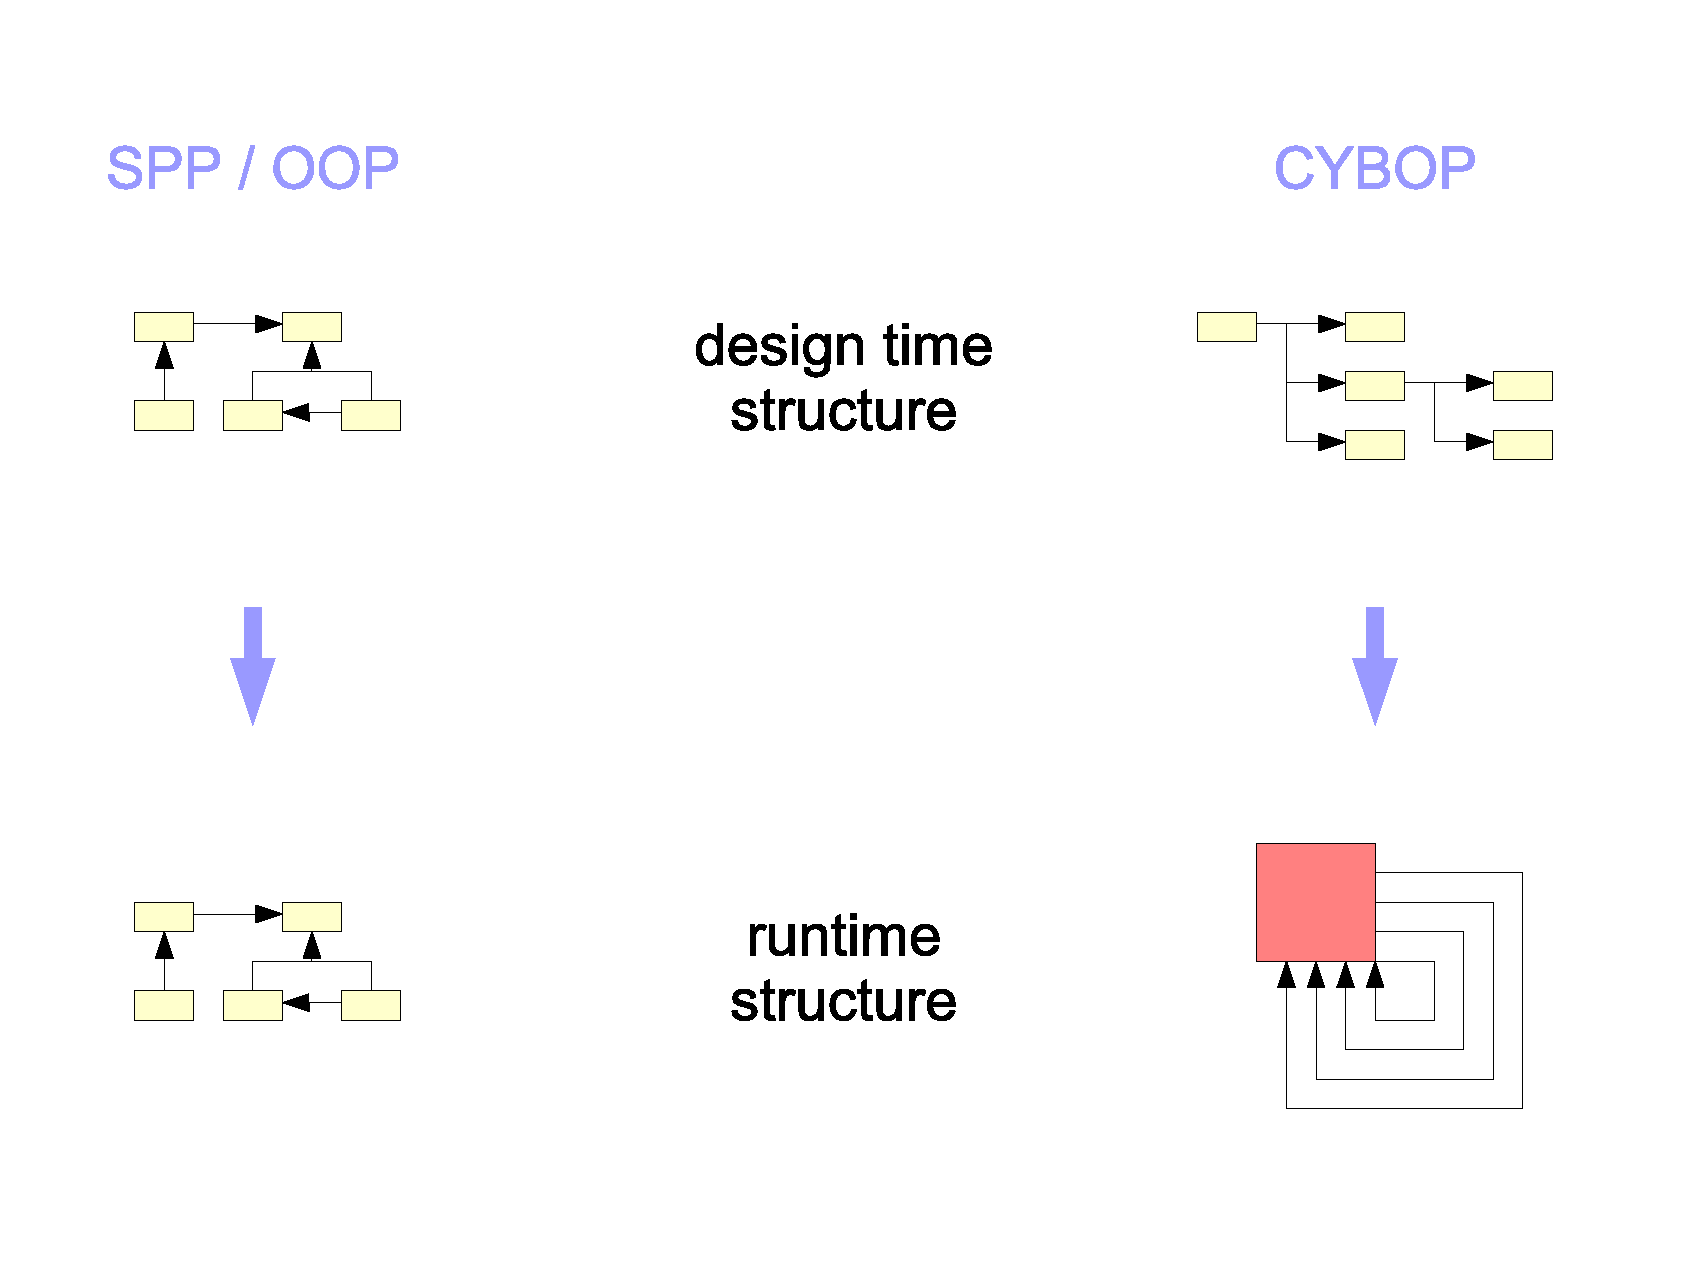
\includegraphics[scale=0.2]{vector/universal.eps}
        \caption{Universal Memory Structure}
        \label{universal_figure}
    \end{center}
\end{figure}

Not so in \emph{Cybernetics Oriented Programming} (CYBOP). Knowledge templates
as created at design time do always have a hierarchical structure, as shown on
the upper right-hand side in the figure. They include \emph{Whole-Part-} as
well as \emph{Meta Hierarchies} (the latter neglected in the figure). At
runtime, these templates get cloned by creating models that follow the
structure of the CYBOP \emph{Knowledge Schema}, as shown on the lower
right-hand side in the figure. While SPP/ OOP rely on a variety of different
structures to store knowledge in memory, CYBOP uses one
\emph{Universal Memory Structure} (knowledge schema) that, so to say, merges
traditional structures like different kinds of \emph{Containers}, \emph{Class}
and \emph{Record}/\emph{Struct}. Even algorithmic structures (logic)
traditionally stored in a \emph{Procedure} are covered by this knowledge
schema. More on state and logic in the following section.

The advantages are obvious. Data available in a unified structure are easier to
process. Dependencies of the knowledge schema are defined clearly and remain
the same for all applications, so that domain/ application knowledge becomes
independent from the underlying system control software. Global data access and
bidirectional dependencies are not necessary anymore, since every knowledge
model can be accessed along well-defined paths within the knowledge hierarchy.
Byte code manipulation and similar tricks and workarounds might finally belong
to the past.
